% 11. előadás

\chapter{Folyamat szinten párhuzamos architektúrák}

\section{Bevezetés}
A folyamat szinten párhuzamos architektúrák MIMD típusúak, multiprocesszoros rendszerek.

\section{Fejlesztési motivációk}
A multiprocesszoros, folyamat szinten párhuzamos rendszerek kifejlesztését az alábbi tényezők tették szükségessé:
\begin{itemize}
    \item Utasítás szintű párhuzamosság korlátozott lehetőségei:
    \begin{itemize}
        \item Branch prediction soha nem 100\%-os.
        \item Általános célú alkalmazásoknál a programokban lévő utasítás szintű párhuzamosság sokszor ahhoz sem elegendő, hogy 4-6 független végrehajtó egységet ellásson utasításokkal.
    \end{itemize}
    \item Energiahatékonyság: egyes CPU-knál kb. 10-15\% számítási teljesítmény növekedéshez akár 50\% fogyasztás emelkedés is szükséges lehet. Következmény, hogy hatékonyabb lehet n darab CPU-t használni egységnyi órajelen, mint 1 darab CPU-t n-szeres órajelen (jól párhuzamosítható feladatok esetén).
    \item Költséghatékonyság: n darab olcsóbb és lassabb CPU összekapcsolása hatékonyabb lehet, mint 1 darab gyors és drága processzor.
    \item Egyszerű bővíthetőség: ha megfelelően fel van készítve, a bővítése könnyebb lehet egy multiprocesszoros rendszernek.
    \item Hibatűrés: ha az egyik processzor meghibásodik, a többi átveszi a feladatait.
\end{itemize}

\section{Csoportosítás}
\subsection{Memória használat szerint}
\begin{itemize}
    \item Közös memória használatú: van olyan, minden CPU számára látható közös memória, melyen keresztül a folyamatok kommunikálni tudnak egymással.
    \item Elosztott memória használatú: a folyamatok üzenetek segítségével kommunikálnak egymással. Ezek az üzenetküldésen alapuló multiprocesszoros rendszerek.
\end{itemize}
\subsection{Memória elérés ideje szerint}
\begin{itemize}
    \item UMA (Uniform Memory Access): a memória elérés ideje azonos minden CPU számára. Következmény, hogy nincs jelentősége annak, hogy a memóriában hova írjuk az adatot.
    \item NUMA (Non-Uniform Memory Access): a memória műveletek ideje nem azonos. Ezeknél a rendszereknél fontos, hogy egy adat az őt író és az őt olvasó CPU-hoz is közel legyen.
\end{itemize}

\section{Korlátok}
\begin{itemize}
    \item Szoftver: vezérlés áramlásos rendszerekben a párhuzamosságok felderítését szoftveresen kell megoldani. Megoldás:
    \begin{itemize}
        \item olyan compilert írunk, ami képes felfedezni a szoftverek párhuzamosítható részeit és ennek megfelelő kódot generál, vagy
        \item a párhuzamosítást a programozóra bízzuk (főleg ez a működőképesebb).
    \end{itemize}
\end{itemize}

\section{Amdahl törvénye}
Annak eldöntéséhez, hogy érdemes-e folyamat szintű párhuzamosítást alkalmazni, felhasználhatjuk Amdahl törvényét.
Segítségével kiszámolható, hogy az n darab CPU-ból álló rendszer mekkora teljesítmény növekedést tud nyújtani.
Ehhez fontos tudni, hogy milyen mértékben párhuzamosíthatók a folyamatok.
Egy valós program tartalmaz szekvenciális és párhuzamosan futtatható részeket is, ezek alapján pedig feltételezhetjük, hogy egy program P-ed része párhuzamosítható.
Ebből következik, hogy 1-P rész szekvenciálisan futtatható.
Legyen a futási idő 1 darab CPU-n 1 egység.
Ekkor N db CPU esetén a futási idő ideális körülmények között:
\begin{center}
    $(1-P)+\dfrac{P}{N}$ .
\end{center}
Ebből a teljesítmény növekedés:
\begin{center}
    $S\textsubscript{p}(N)=\dfrac{1}{1-P+\dfrac{P}{N}}$ .
\end{center}
Például, ha azt szeretnénk, hogy egy 100 processzoros rendszeren 50-szeres teljesítmény növekedést kapjunk az 1 CPU-hoz képest, akkor
\begin{center}
    $P=\dfrac{S\textsubscript{p}(N)-1}{S\textsubscript{p}(N)}\cdot\dfrac{N}{N-1}\approx0.9898$ ,
\end{center}
tehát a programunk majdnem 100\%-ának párhuzamosíthatónak kell lennie.
Amdahl törvényéből következik, hogy a gyorsulásnak véges határértéke lesz végtelen processzor esetén is, mivel
\begin{center}
    $\displaystyle{\lim_{N \to \infty}}S\textsubscript{p}(N)=\dfrac{1}{1-P}$ ,
\end{center}
így például egy 95\%-ban párhuzamosítható programmal legfeljebb 20-szoros gyorsulás érhető el.
Következmény: a processzorok számát nem gazdaságos egy bizonyos határon túl emelni.

\section{UMA rendszerek}
\subsection{Felépítés}
Az UMA, vagy más néven SMP (Symmetric Multiprocessing) rendszereknél a processzorok egy közös buszon keresztül érik el a memóriát (\ref{fig:uma}. ábra).
Probléma, hogy a közös buszrendszeren keresztül továbbítódik minden adat, így az szűk keresztmetszetet képez.
Ezért a megoldás nem jól skálázható, kb. 8-16 CPU köthető össze a buszrendszer túlterhelése nélkül.
\begin{figure}[H]
    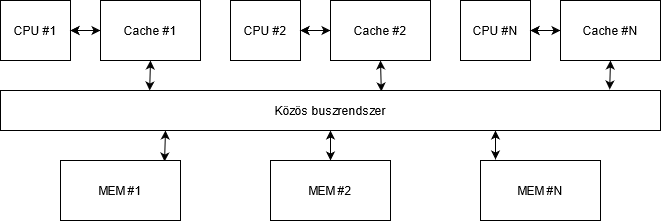
\includegraphics[width=\textwidth]{uma}
    \centering
    \caption{Az UMA rendszerek memória elérése}
    \label{fig:uma}
\end{figure}
\subsection{Gyakorlati példa}
A kezdeti többmagos architektúráknál alkalmazott FSB (Front Side Bus) felépítés UMA elven működik (\ref{fig:fsb}. ábra).
\begin{figure}[H]
    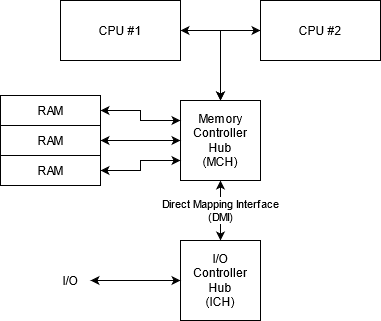
\includegraphics[width=0.6\textwidth]{fsb}
    \centering
    \caption{A tradícionális FSB rendszer felépítése}
    \label{fig:fsb}
\end{figure}

\section{NUMA rendszerek}
\subsection{Felépítés}
Az UMA rendszerek problémáinak kiküszöbölésére fejlesztették a NUMA architektúrákat, amik közös, de tartományokra bontott memória címtérrel rendelkeztek (\ref{fig:numa}. ábra).
A tartományok megfelelői az ábrán a csomópontok.
Eredmény, hogy a buszrendszerre kisebb terhelés esik, így a megoldás jól skálázható.
\begin{figure}[H]
    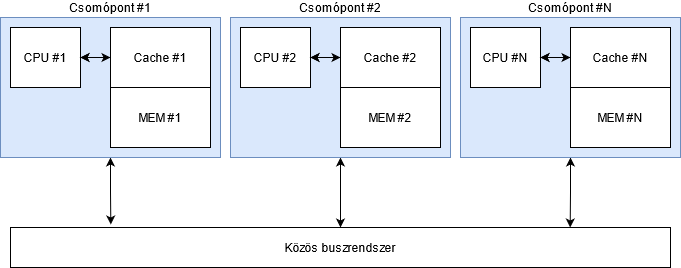
\includegraphics[width=\textwidth]{numa}
    \centering
    \caption{A NUMA rendszerek memória elérése}
    \label{fig:numa}
\end{figure}
\subsection{Csoportosítás}
A NUMA rendszereket két csoportra oszthatjuk:
\begin{itemize}
    \item CC NUMA: cache coherent
    \item NC NUMA: non cache coherent
\end{itemize}

\subsection{Cache coherent}
A cache koherens rendszereknél az adatok legfrissebb példányát a gyorsítótárakban nyilvántartják és frissítik.
Ez a gyakorlatban azt jelenti, hogy ha két CPU ugyanazzal az adattal dolgozna, és mindkettő betölti a gyorsítótárába, majd az egyik módosítja az adatot, a másik CPU gyorsítótárában lévő adatot invalidálja egy figyelő rendszer és az adat frissítésre kerül.
A módszer hátránya, hogy ez komoly adminisztrációt igényel, ami a buszrendszert terheli.
A CC NUMA rendszereket ezért szokás hívni az UMA rendszerek skálázható kiterjesztésének is.
Ez a megoldás kb. 32 CPU-ig skálázható, viszont az UMA-hoz képest a memória műveletek késleltetése 2-7-szeresére növekszik.

\subsection{Non cache coherent}
A nem cache koherens rendszerek nem garantálják, hogy a proceszor mindig az adat legfrissebb verziójával dolgozik, az ebből adódó problémás helyzeteket szoftveresen kell detektálni és kezelni.
Ez a legjobban skálázható megoldás, tervezése és építése könnyű, viszont a programozása sokkal nehezebb.
Általában sok gépes (több összekapcsolt szerver) rendszerekben használják.
Ilyen processzor például az Intel Xeon és az AMD Opteron.

\subsection{Gyakorlati példák}
\subsubsection{Quick Path Interconnect}
A modern többmagos processzorokban a klasszikus FSB felépítés helyett a QPI (Quick Path Interconnect) technológiát használják, ahol a CPU-k egy nagy sebességű buszon (QPI) kommunikálnak egymással (\ref{fig:qpi}. ábra).
Ennek előnye, hogy a memória kontrollerek a processzorok lapkáira vannak integrálva, így a memória elérése gyorsul.
Mivel így már a CPU-knak külön memóriaterületet kell kezelniük, ez egy NUMA architektúrának számít.
\begin{figure}[H]
    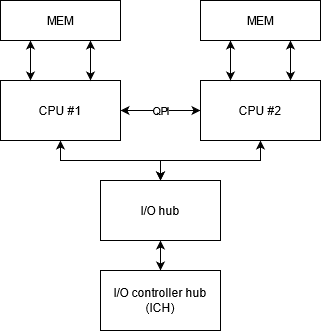
\includegraphics[width=0.5\textwidth]{qpi}
    \centering
    \caption{A Quick Path Interconnect felépítése}
    \label{fig:qpi}
\end{figure}
\subsubsection{Intel Core i}
A mai Core i architektúráknál már a processzorokon belüli magok is eltérő memória területeket kezelnek.
Egy 4 magos CPU-nál két-két mag kap egy közös memóriavezérlőt, a magok pedig egy, a QPI-hez hasonló buszrendszeren kommunikálnak.
A gyors adatelérés érdekében a magok közös L3 cache-t használnak (\ref{fig:corei}. ábra).
\begin{figure}[H]
    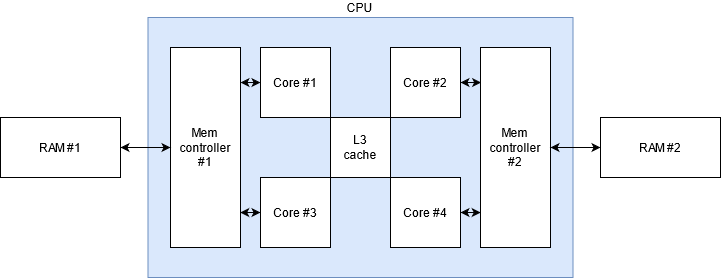
\includegraphics[width=\textwidth]{corei}
    \centering
    \caption{A modern Intel Core i processzorok felépítése}
    \label{fig:corei}
\end{figure}

\section{Összegzés}
A modern több magos és több processzoros rendszerekben inkább NUMA felépítést alkalmaznak.
Az előbb bemutatott Core i processzor is egy példa arra, hogy a nagy, több gépes rendszereken kívül a mikroarchitektúrák szintjén is megtalálhatók a NUMA jellemzők.
A szerverekben cache koherens NUMA rendszerek dominálnak, a nem cache koherens technológiákkal pedig több gépből álló rendszerek építhetők.